\documentclass{article}

\usepackage{amsmath}
\usepackage{amssymb}
\usepackage{graphicx}
\usepackage{caption}
\usepackage{subcaption}
\usepackage{cite}
\usepackage{hyperref}
\usepackage{geometry}
\usepackage{fancyhdr}
\usepackage{setspace}
\usepackage{enumitem}
\usepackage{lipsum}
\usepackage{float}
\usepackage{enumitem}
\usepackage{amsfonts}

\graphicspath{ {./graphs/} }

% Page layout
\geometry{top=1in, bottom=1in, left=1in, right=1in}
\pagestyle{fancy}
\fancyhf{}
\rhead{Matic Stare}
\lhead{Homework 3}
\cfoot{\thepage}
\renewcommand{\headrulewidth}{0.4pt}
\renewcommand{\footrulewidth}{0.4pt}

% Title
\title{Homework 3}
\author{Matic Stare}
\date{\today}

\begin{document}

\maketitle

% Table of Contents
\tableofcontents
\newpage

% Sections
\section{Homology}\label{sec:p1}

\section{Discrete Morse Theory}\label{sec:p2}

\section{Vietoris-Rips complex}\label{sec:p3}

We started this exercise by implementing the cliques function. To optimize it as much as possible, we only checked for every dimension the vertices whose degree is greater or equal to the $\text{dimension} - 1$. Then for every added edge we checked if the construction still forms a clique. We first tested our algorithm on a graph representation of a tetrahedra~\ref{fig:g4}. The evalvation was instant, because there are only 4 vertices and 6 edges. We figured out, that our algorithm runs the worst, when the given input graph is a complete graph. Because of that, we first tested it on a complete graph of 16 vertices~\ref{fig:g16}. The algorithm ran around a second. Then we inputed the complete graph of 19 vertices~\ref{fig:g19}. The algorithm was done in 10 seconds. Lastly, we tried the complete graph of 22 vertices~\ref{fig:g22}. The algorithm finished in around 100 seconds.



\begin{figure}[H]
    \begin{subfigure}{0.495\linewidth}
        \centering
        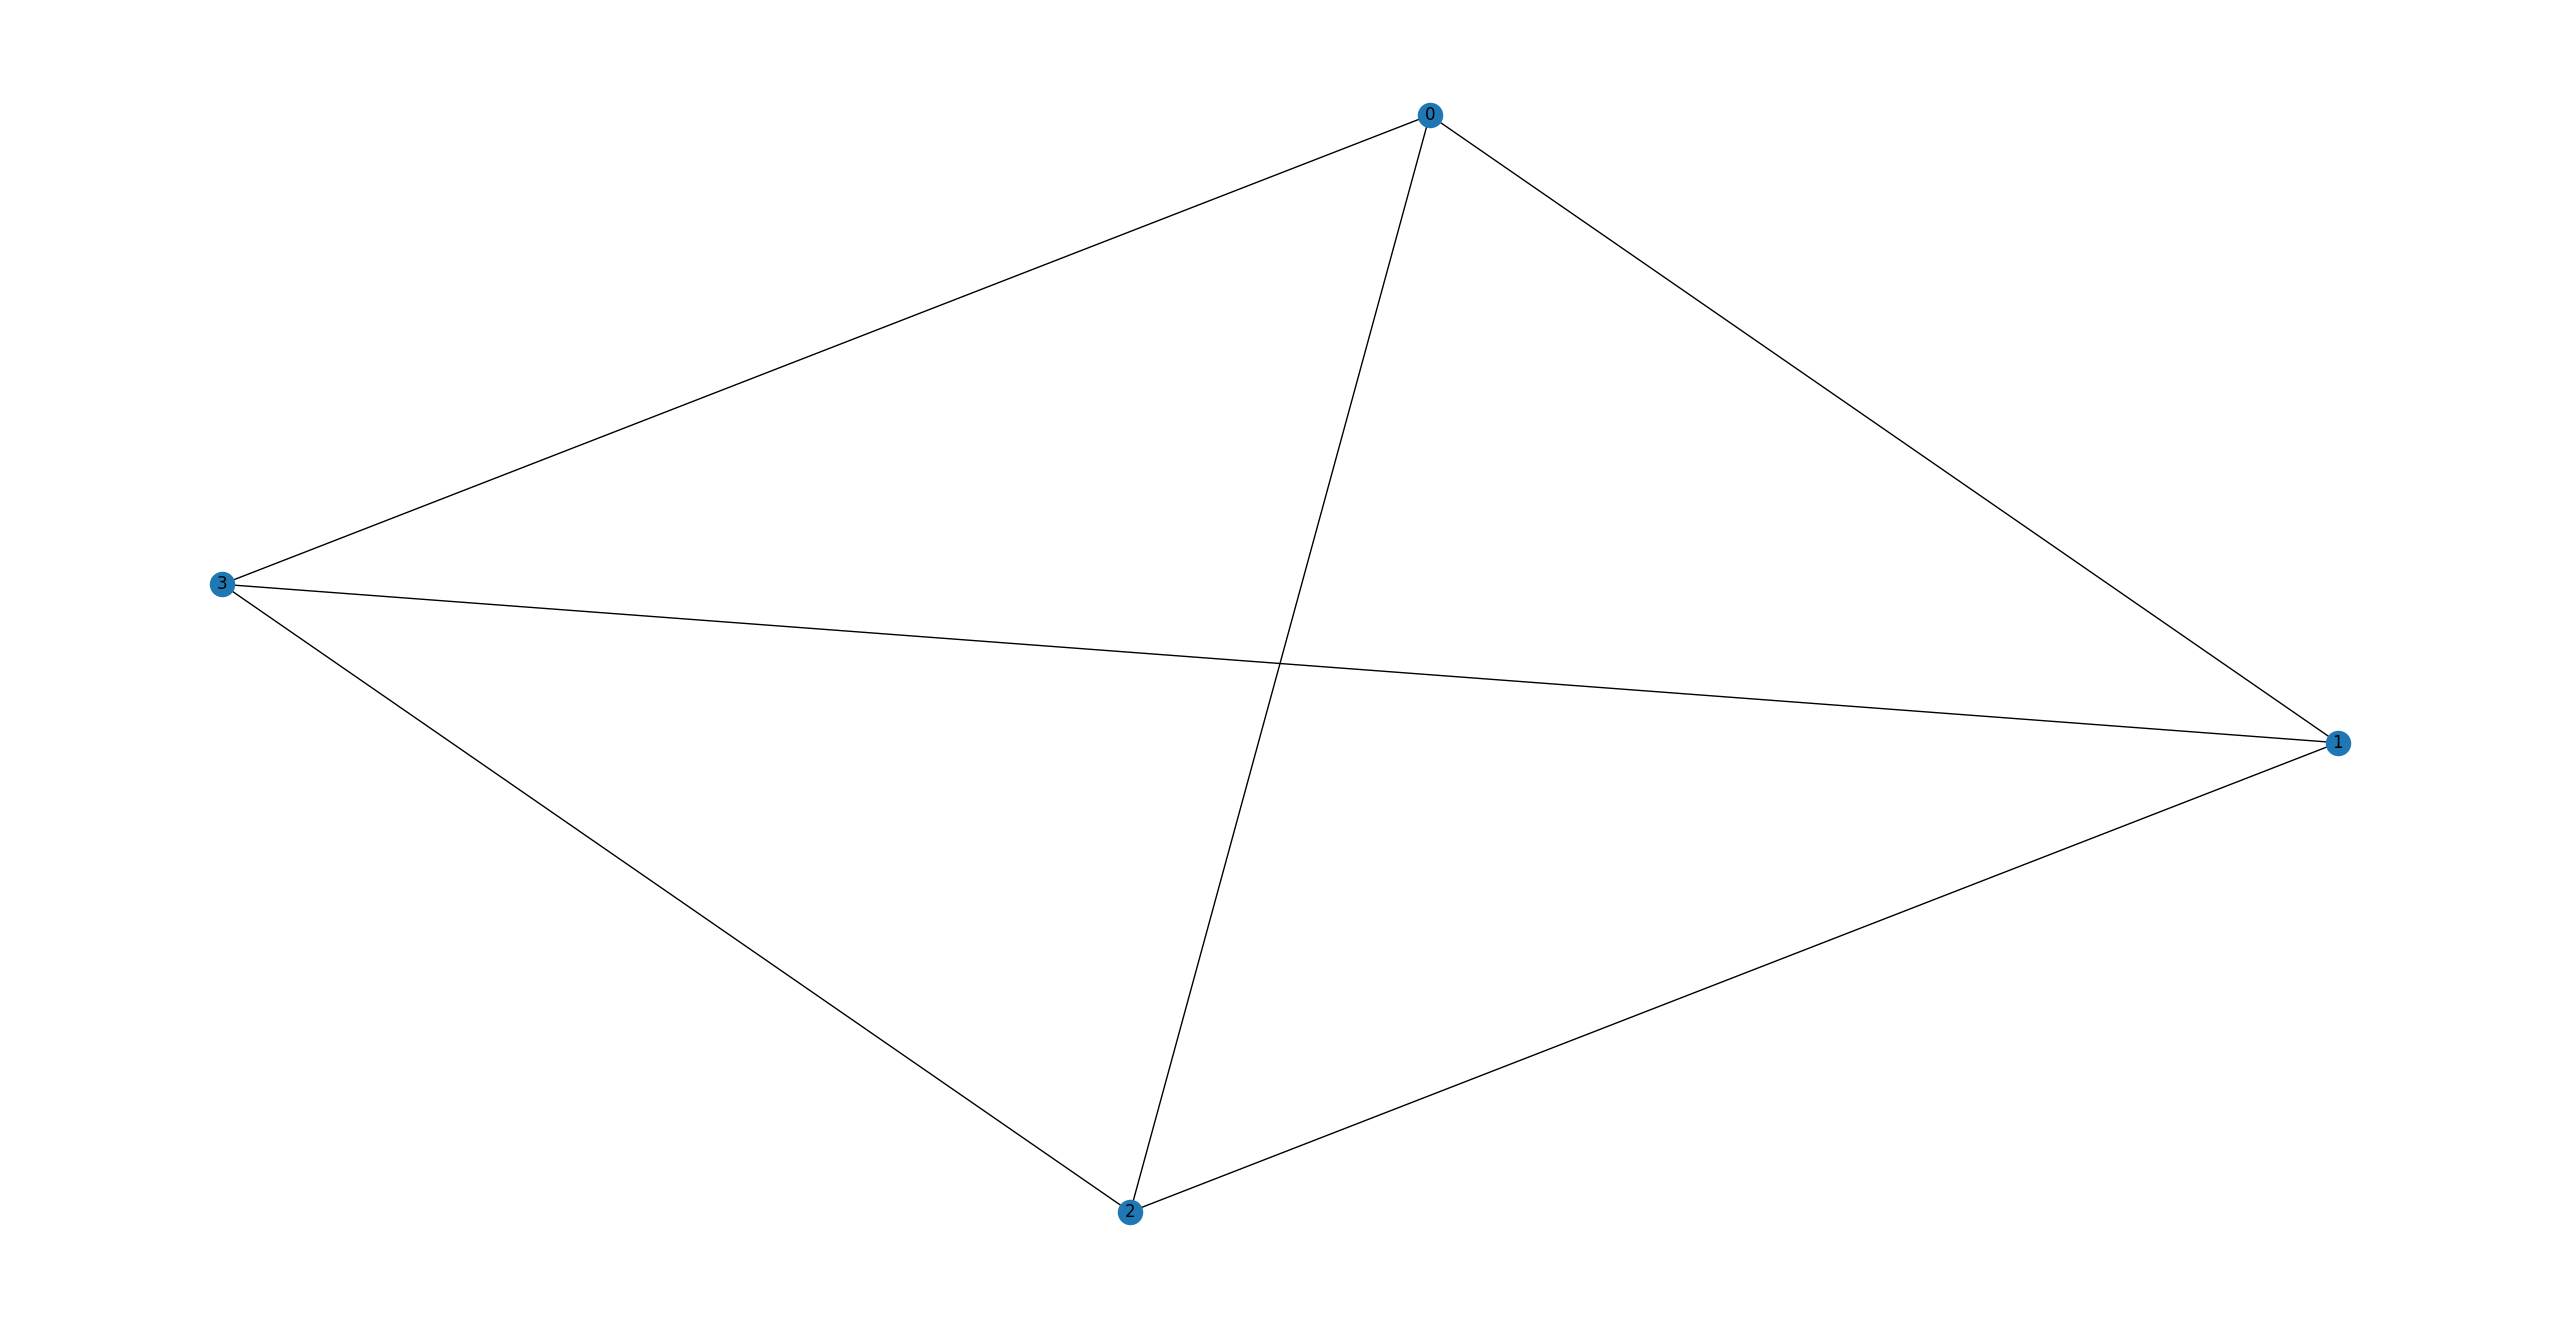
\includegraphics[width=\textwidth]{g4.png}
        \caption{Tetrahedra.}\label{fig:g4}
    \end{subfigure}
    \begin{subfigure}{0.495\linewidth}
        \centering
        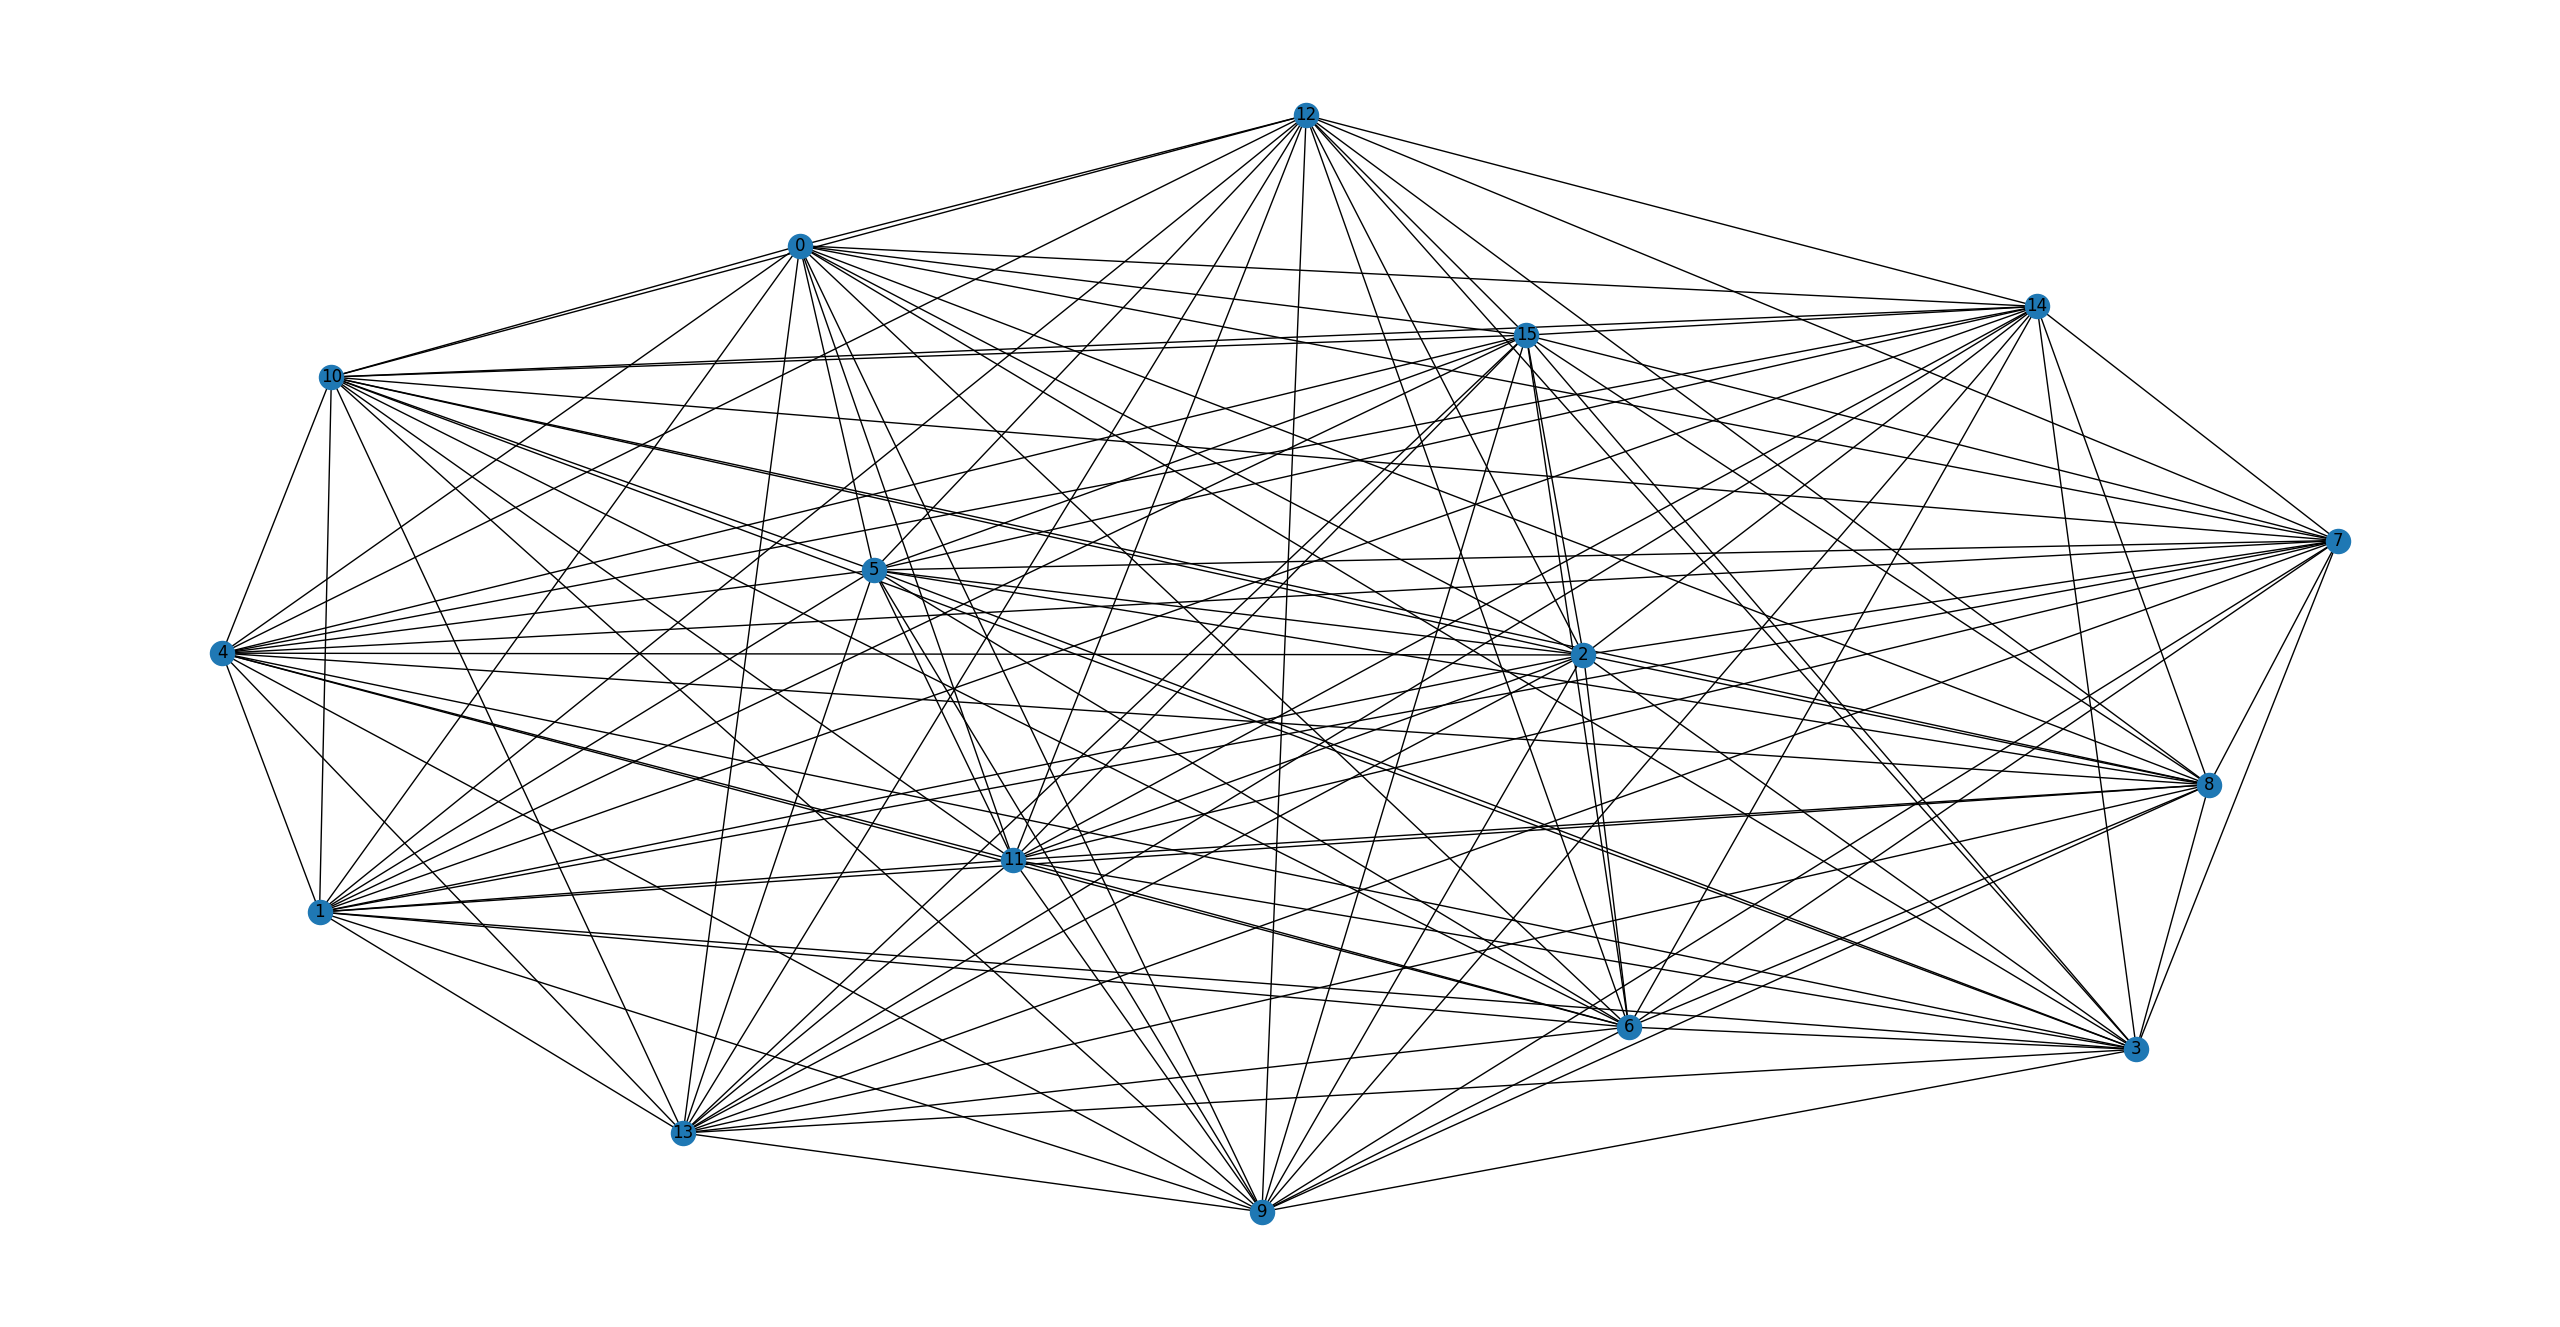
\includegraphics[width=\textwidth]{g16.png}
        \caption{Complete graph on 16 vertices.}\label{fig:g16}
    \end{subfigure}
    \begin{subfigure}{0.495\linewidth}
        \centering
        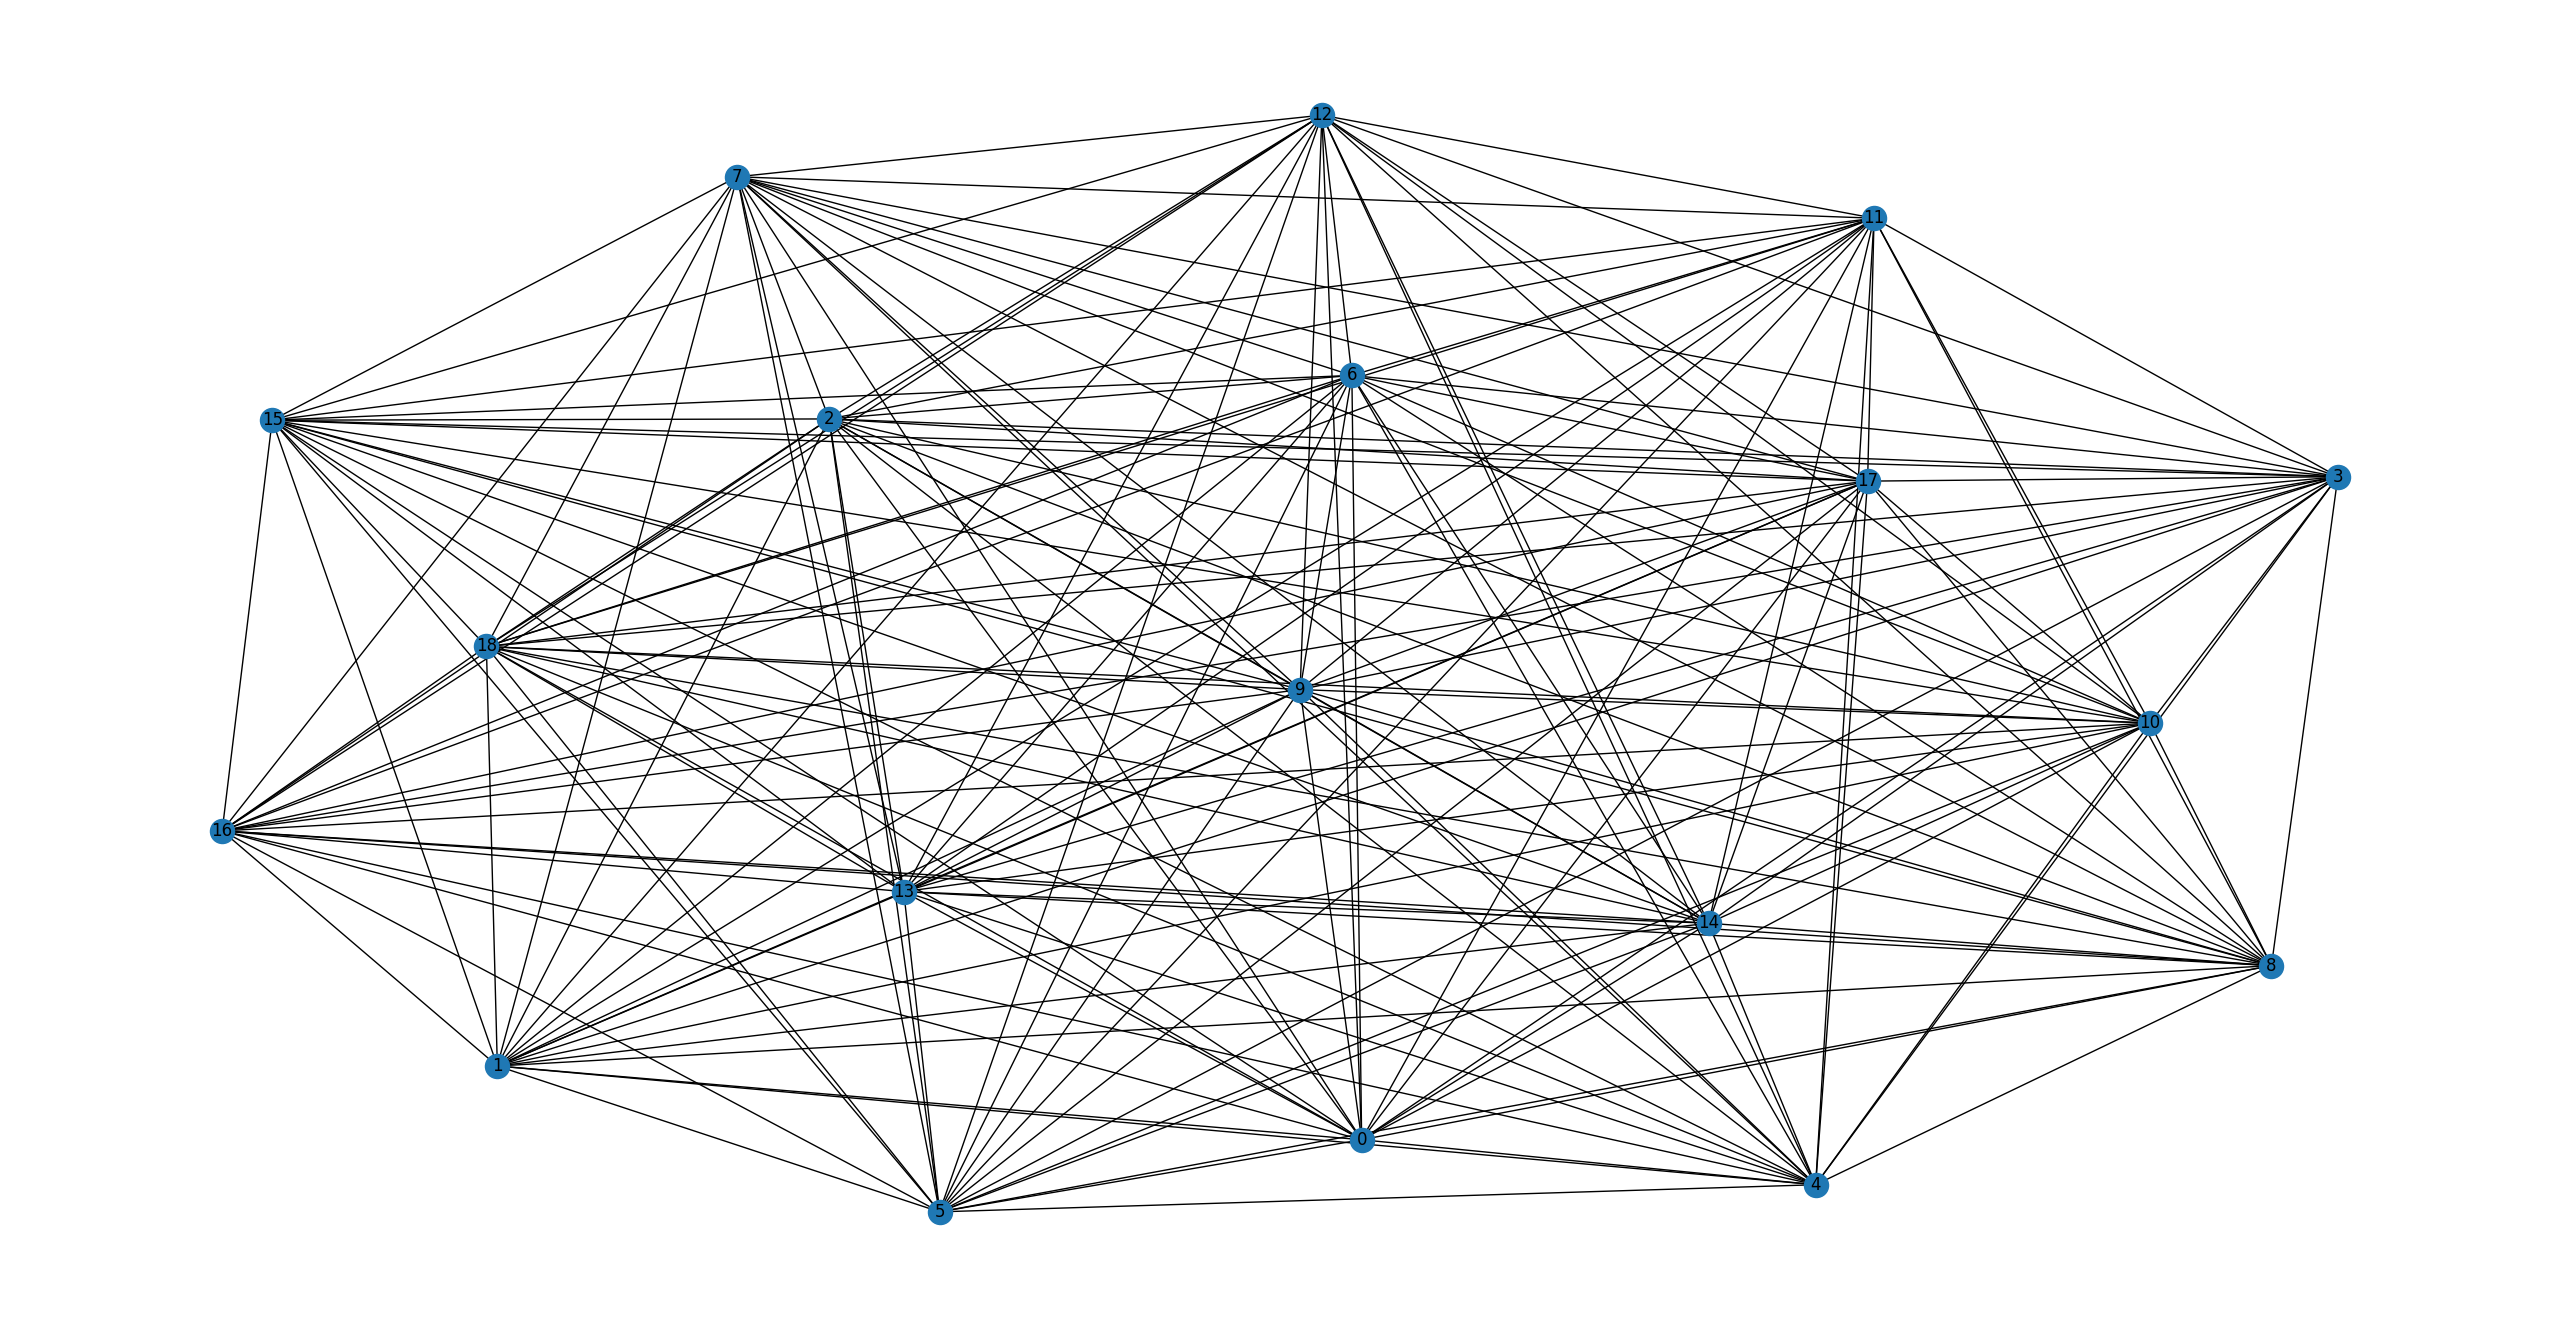
\includegraphics[width=\textwidth]{g19.png}
        \caption{Complete graph on 19 vertices.}\label{fig:g19}
    \end{subfigure}
    \begin{subfigure}{0.495\linewidth}
        \centering
        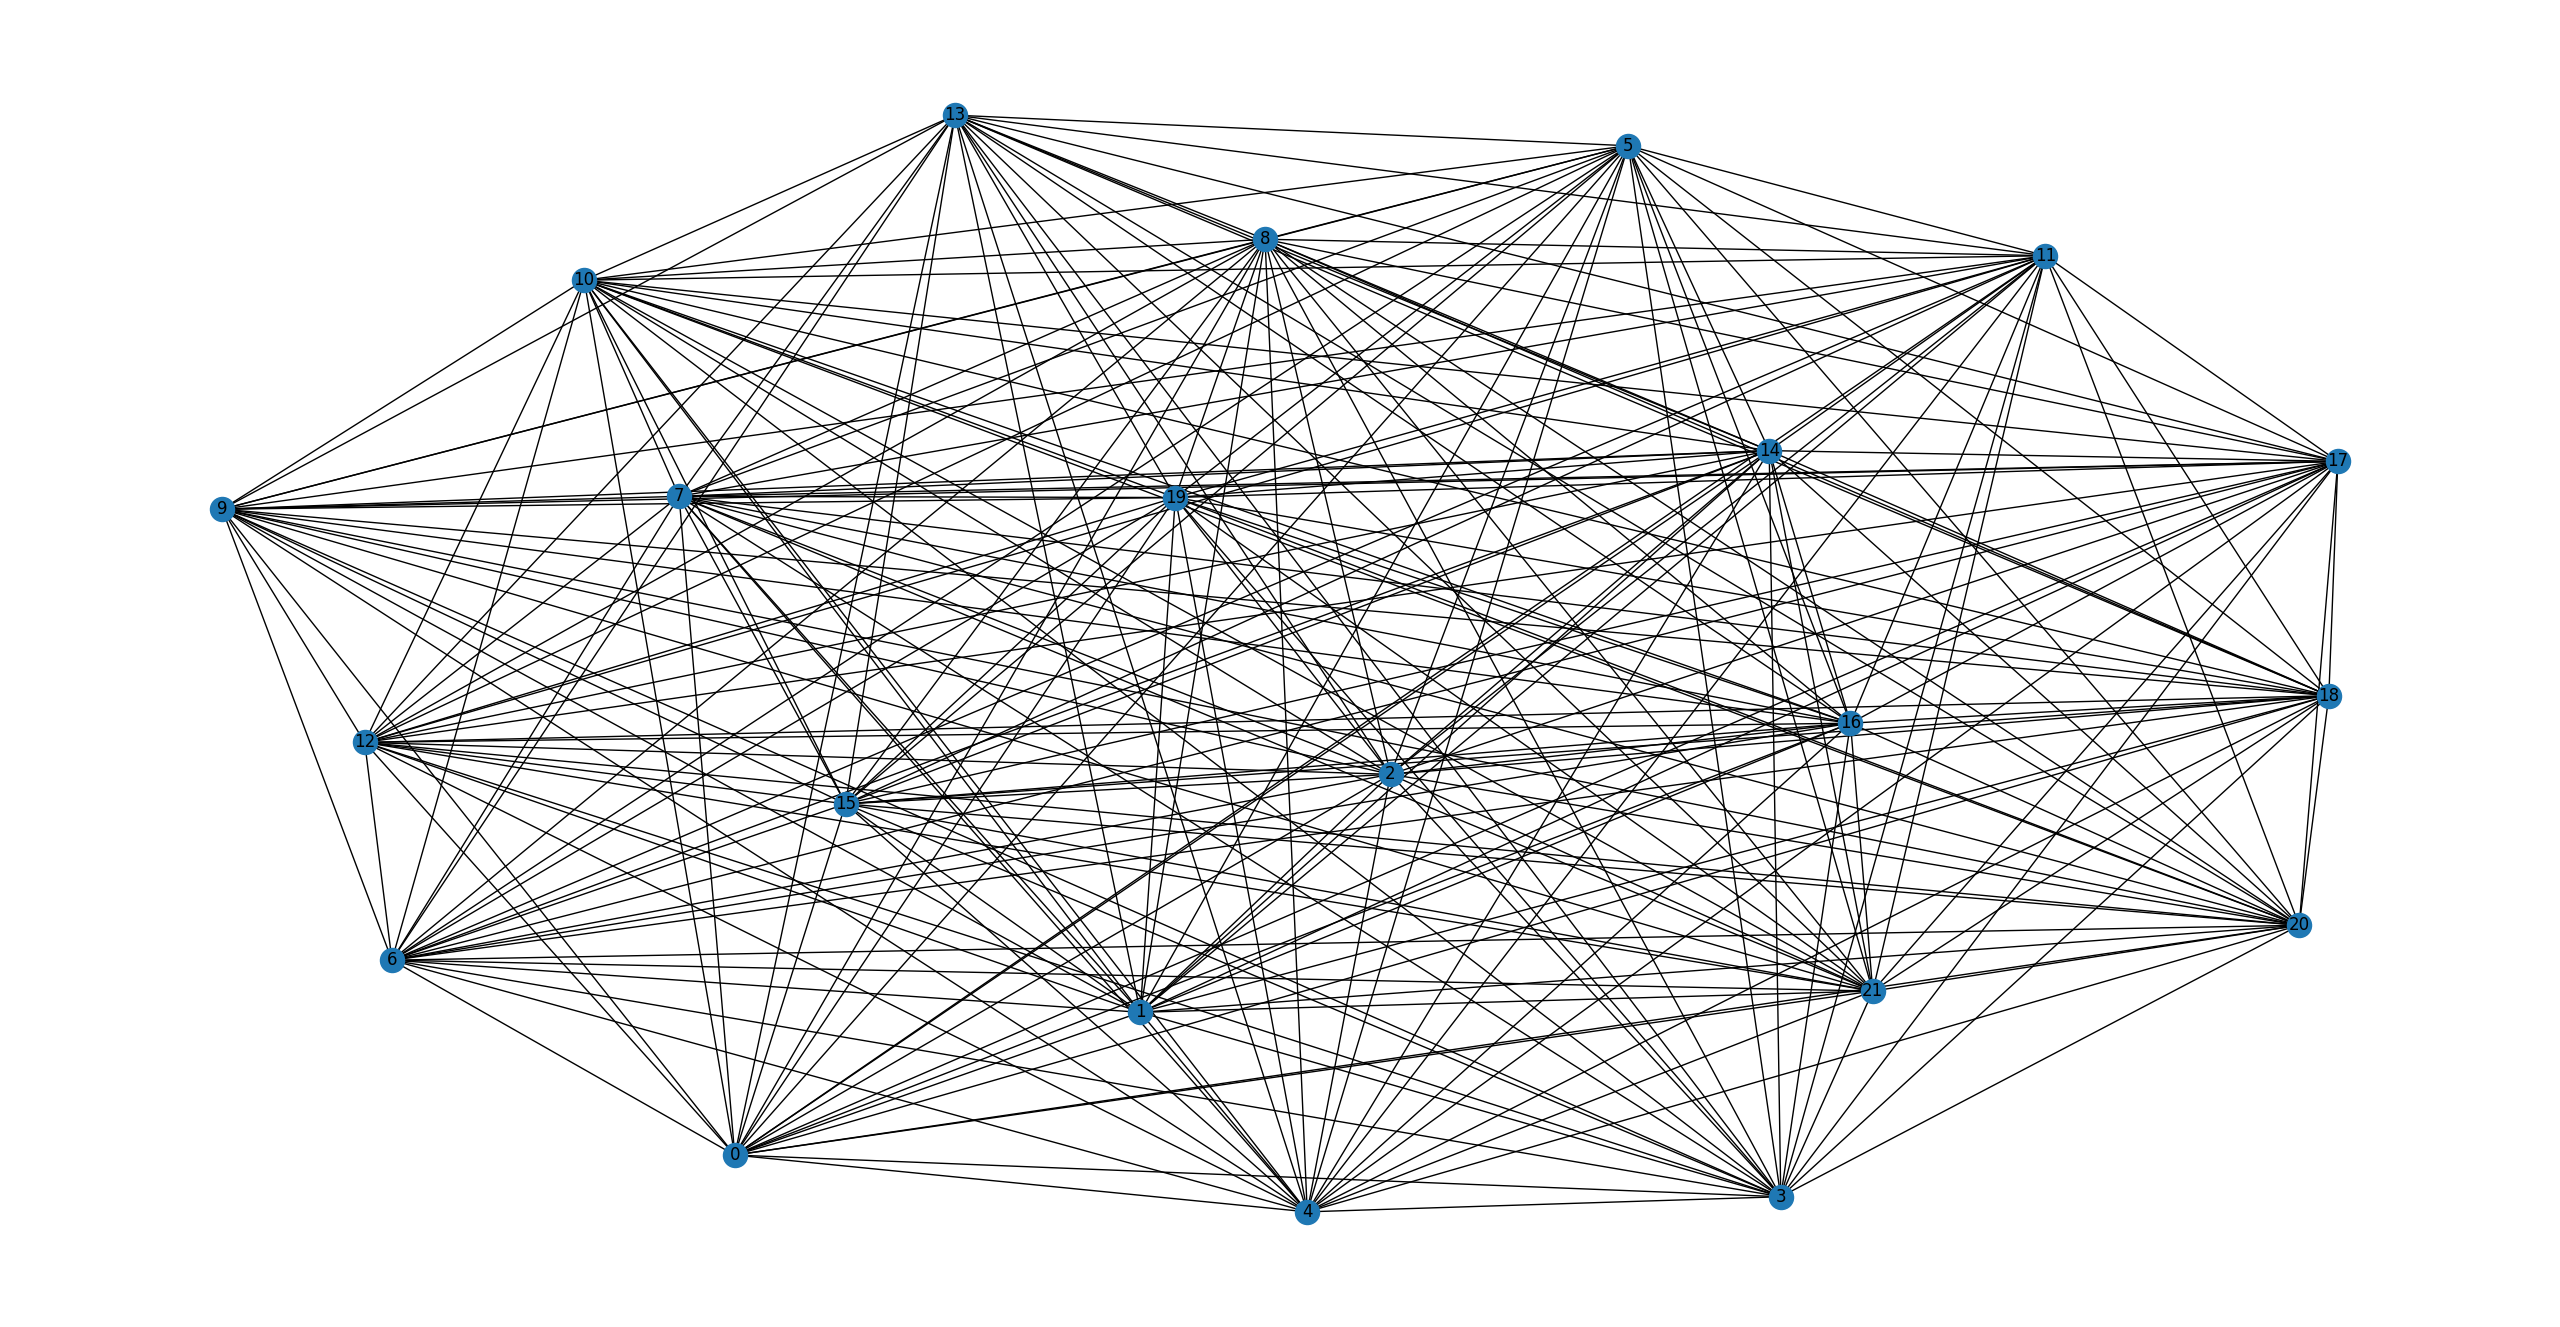
\includegraphics[width=\textwidth]{g22.png}
        \caption{Complete graph on 22 vertices.}\label{fig:g22}
    \end{subfigure}
    \caption{Representation of input data used on cliques algorithm.}\label{fig:cliquesGraphs}
\end{figure}

We continued by implementing Vietoris-Rips complex. We calculated all edges and then used the cliques function to calculate all simplices in every dimension. We tested our algorithm on the given sample~\ref{fig:vr1}. The algorithm returned these simplices:\\
Dimension 0 simplices: [[0], [1], [2], [3], [4], [5]]\\
Dimension 1 simplices: [[0, 1], [0, 3], [1, 2], [1, 3], [1, 4], [2, 5]]\\
Dimension 2 simplices: [[0, 1, 3]]

Then we randomly generated a graph with 10 vertices~\ref{fig:vr2}. The algorithm returned these simplices:\\
Dimension 0 simplices: [[0], [1], [2], [3], [4], [5], [6], [7], [8], [9]]\\
Dimension 1 simplices: [[0, 4], [1, 5], [1, 7], [2, 6], [2, 8], [2, 9], [3, 9], [5, 7], [6, 8], [6, 9], [8, 9]]\\
Dimension 2 simplices: [[1, 5, 7], [2, 6, 8], [2, 6, 9], [2, 8, 9], [6, 8, 9]]\\
Dimension 3 simplices: [[2, 6, 8, 9]]

Lastly, we randomly generated a graph with 20 vertices~\ref{fig:vr3}. The algorithm returned these simplices:\\
Dimension 0 simplices: [[0], [1], [2], [3], [4], [5], [6], [7], [8], [9], [10], [11], [12], [13], [14], [15], [16], [17], [18], [19]]\\
Dimension 1 simplices: [[0, 5], [0, 13], [0, 14], [0, 15], [1, 7], [1, 19], [2, 4], [2, 14], [3, 9], [3, 11], [3, 16], [4, 14], [5, 8], [5, 13], [5, 15], [5, 17], [5, 18], [6, 10], [6, 12], [7, 16], [8, 17], [8, 18], [9, 11], [9, 16], [10, 12], [10, 19], [11, 16], [13, 15], [13, 17], [14, 15], [17, 18]]\\
Dimension 2 simplices: [[0, 5, 13], [0, 5, 15], [0, 13, 15], [0, 14, 15], [2, 4, 14], [3, 9, 11], [3, 9, 16], [3, 11, 16], [5, 8, 17], [5, 8, 18], [5, 13, 15], [5, 13, 17], [5, 17, 18], [6, 10, 12], [8, 17, 18], [9, 11, 16]]\\
Dimension 3 simplices: [[0, 5, 13, 15], [3, 9, 11, 16], [5, 8, 17, 18]]

\begin{figure}[H]
    \begin{subfigure}{0.33\linewidth}
        \centering
        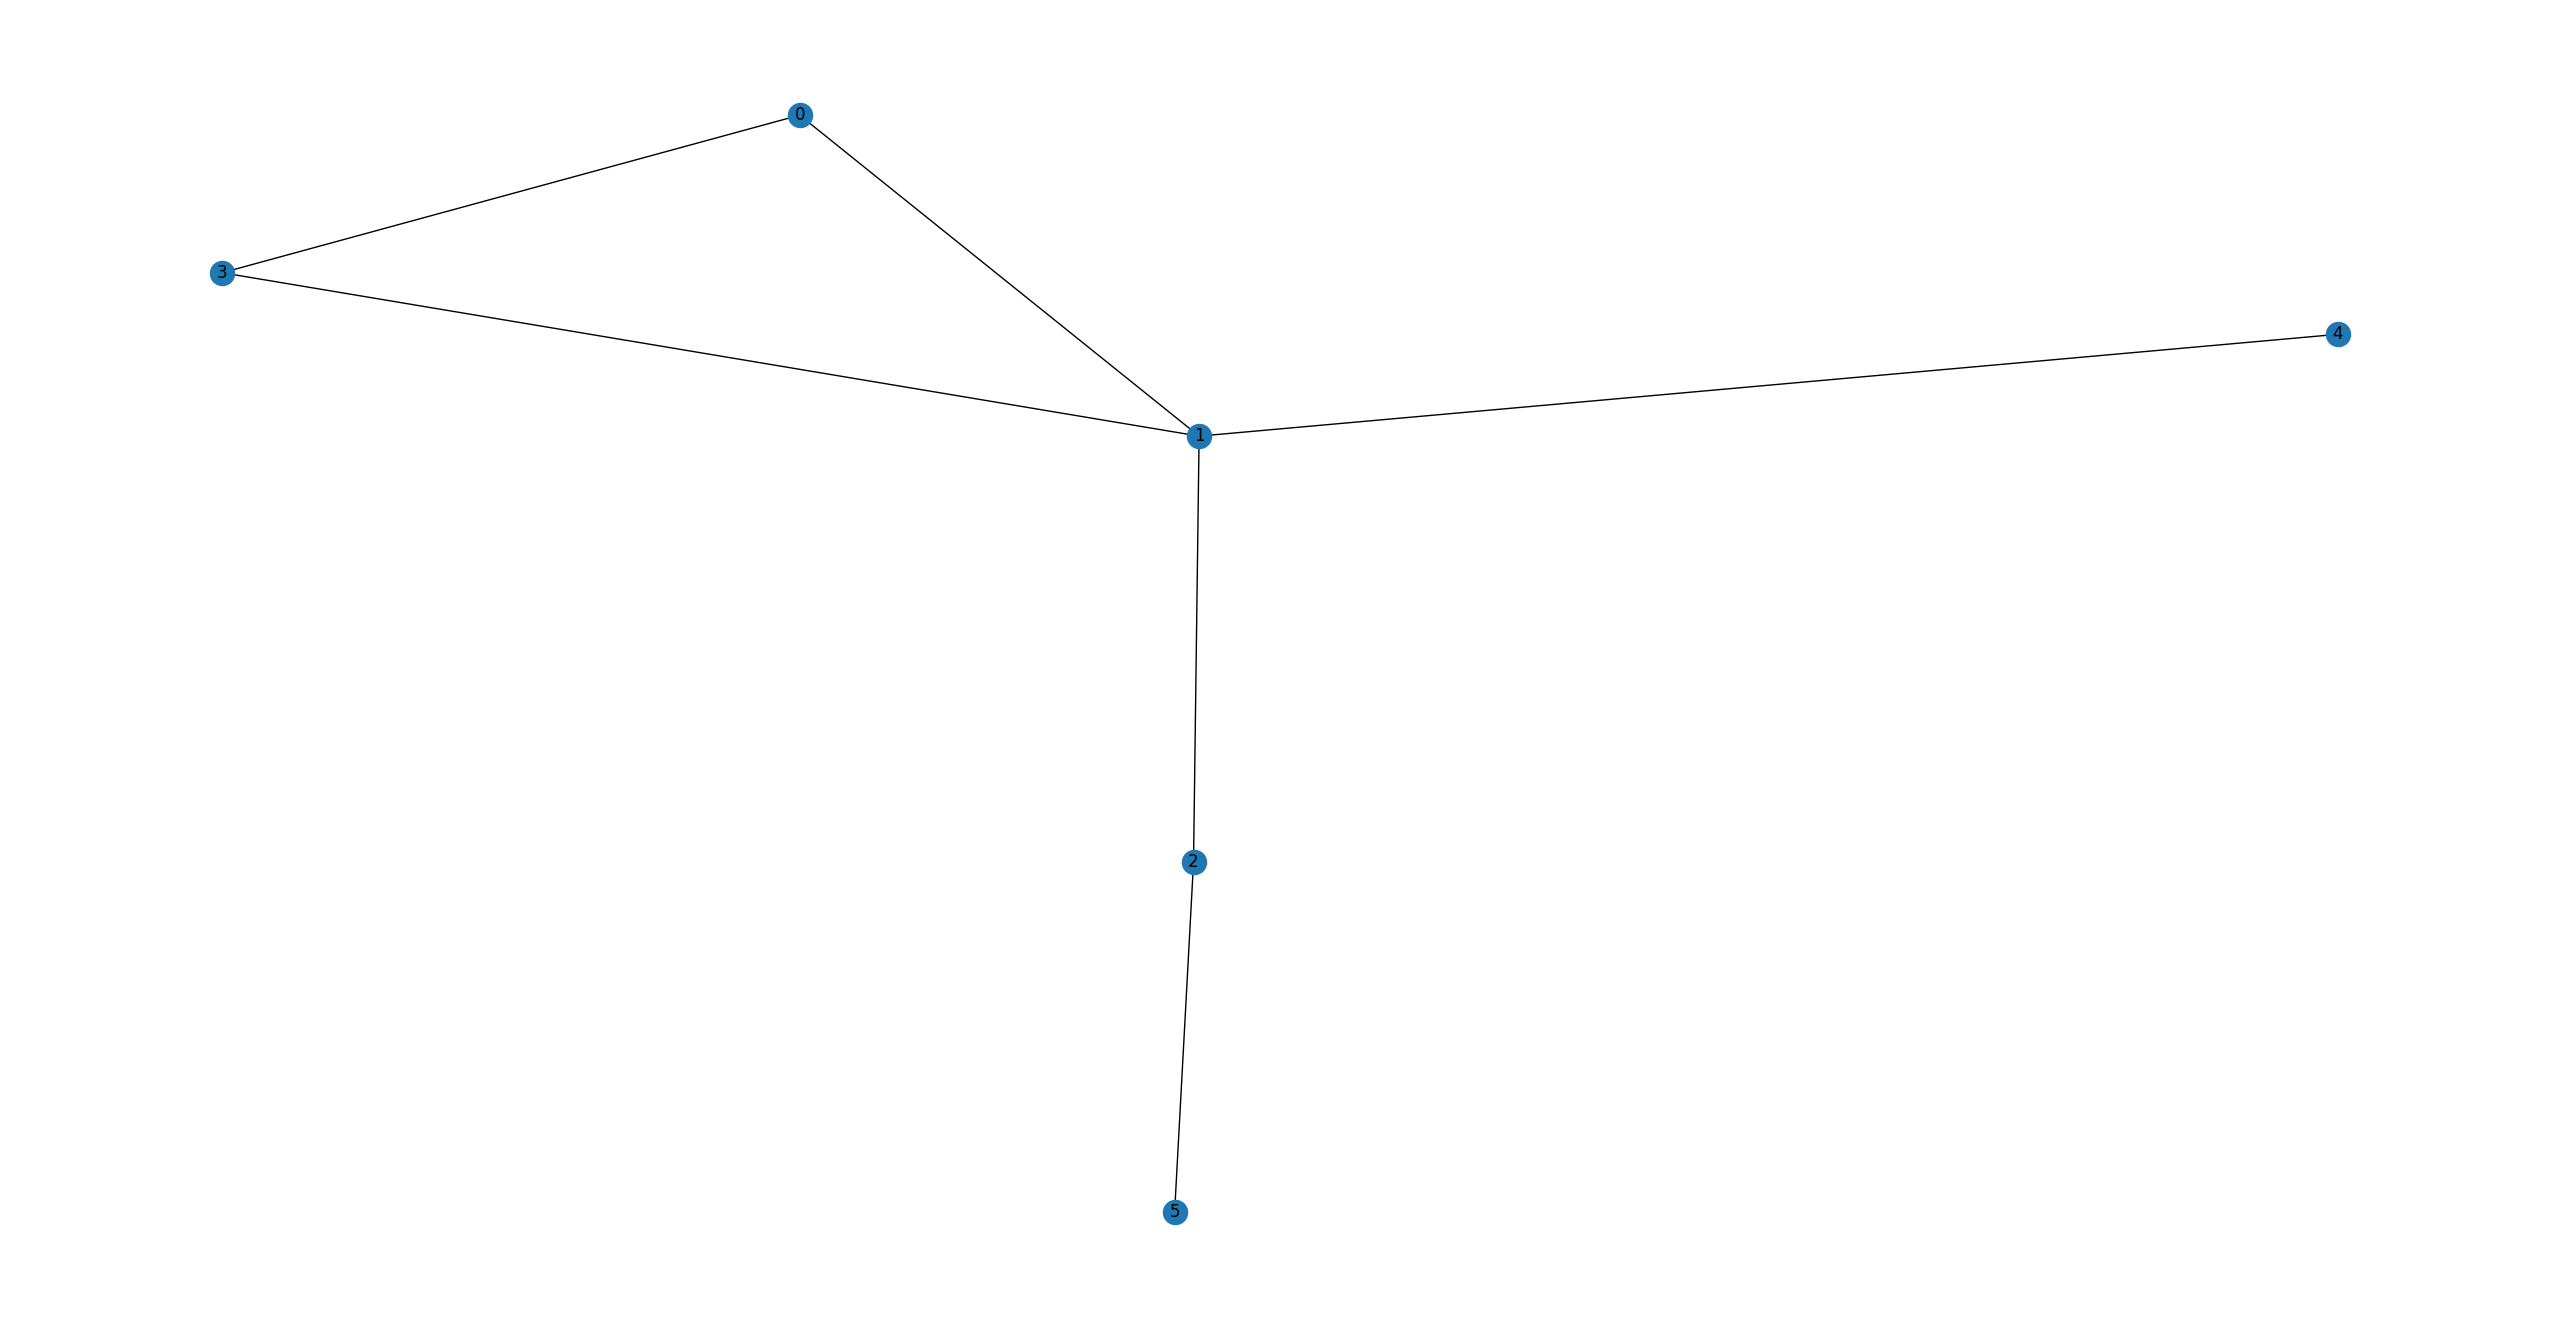
\includegraphics[width=\textwidth]{vr1.png}
        \caption{Given sample graph.}\label{fig:vr1}
    \end{subfigure}
    \begin{subfigure}{0.33\linewidth}
        \centering
        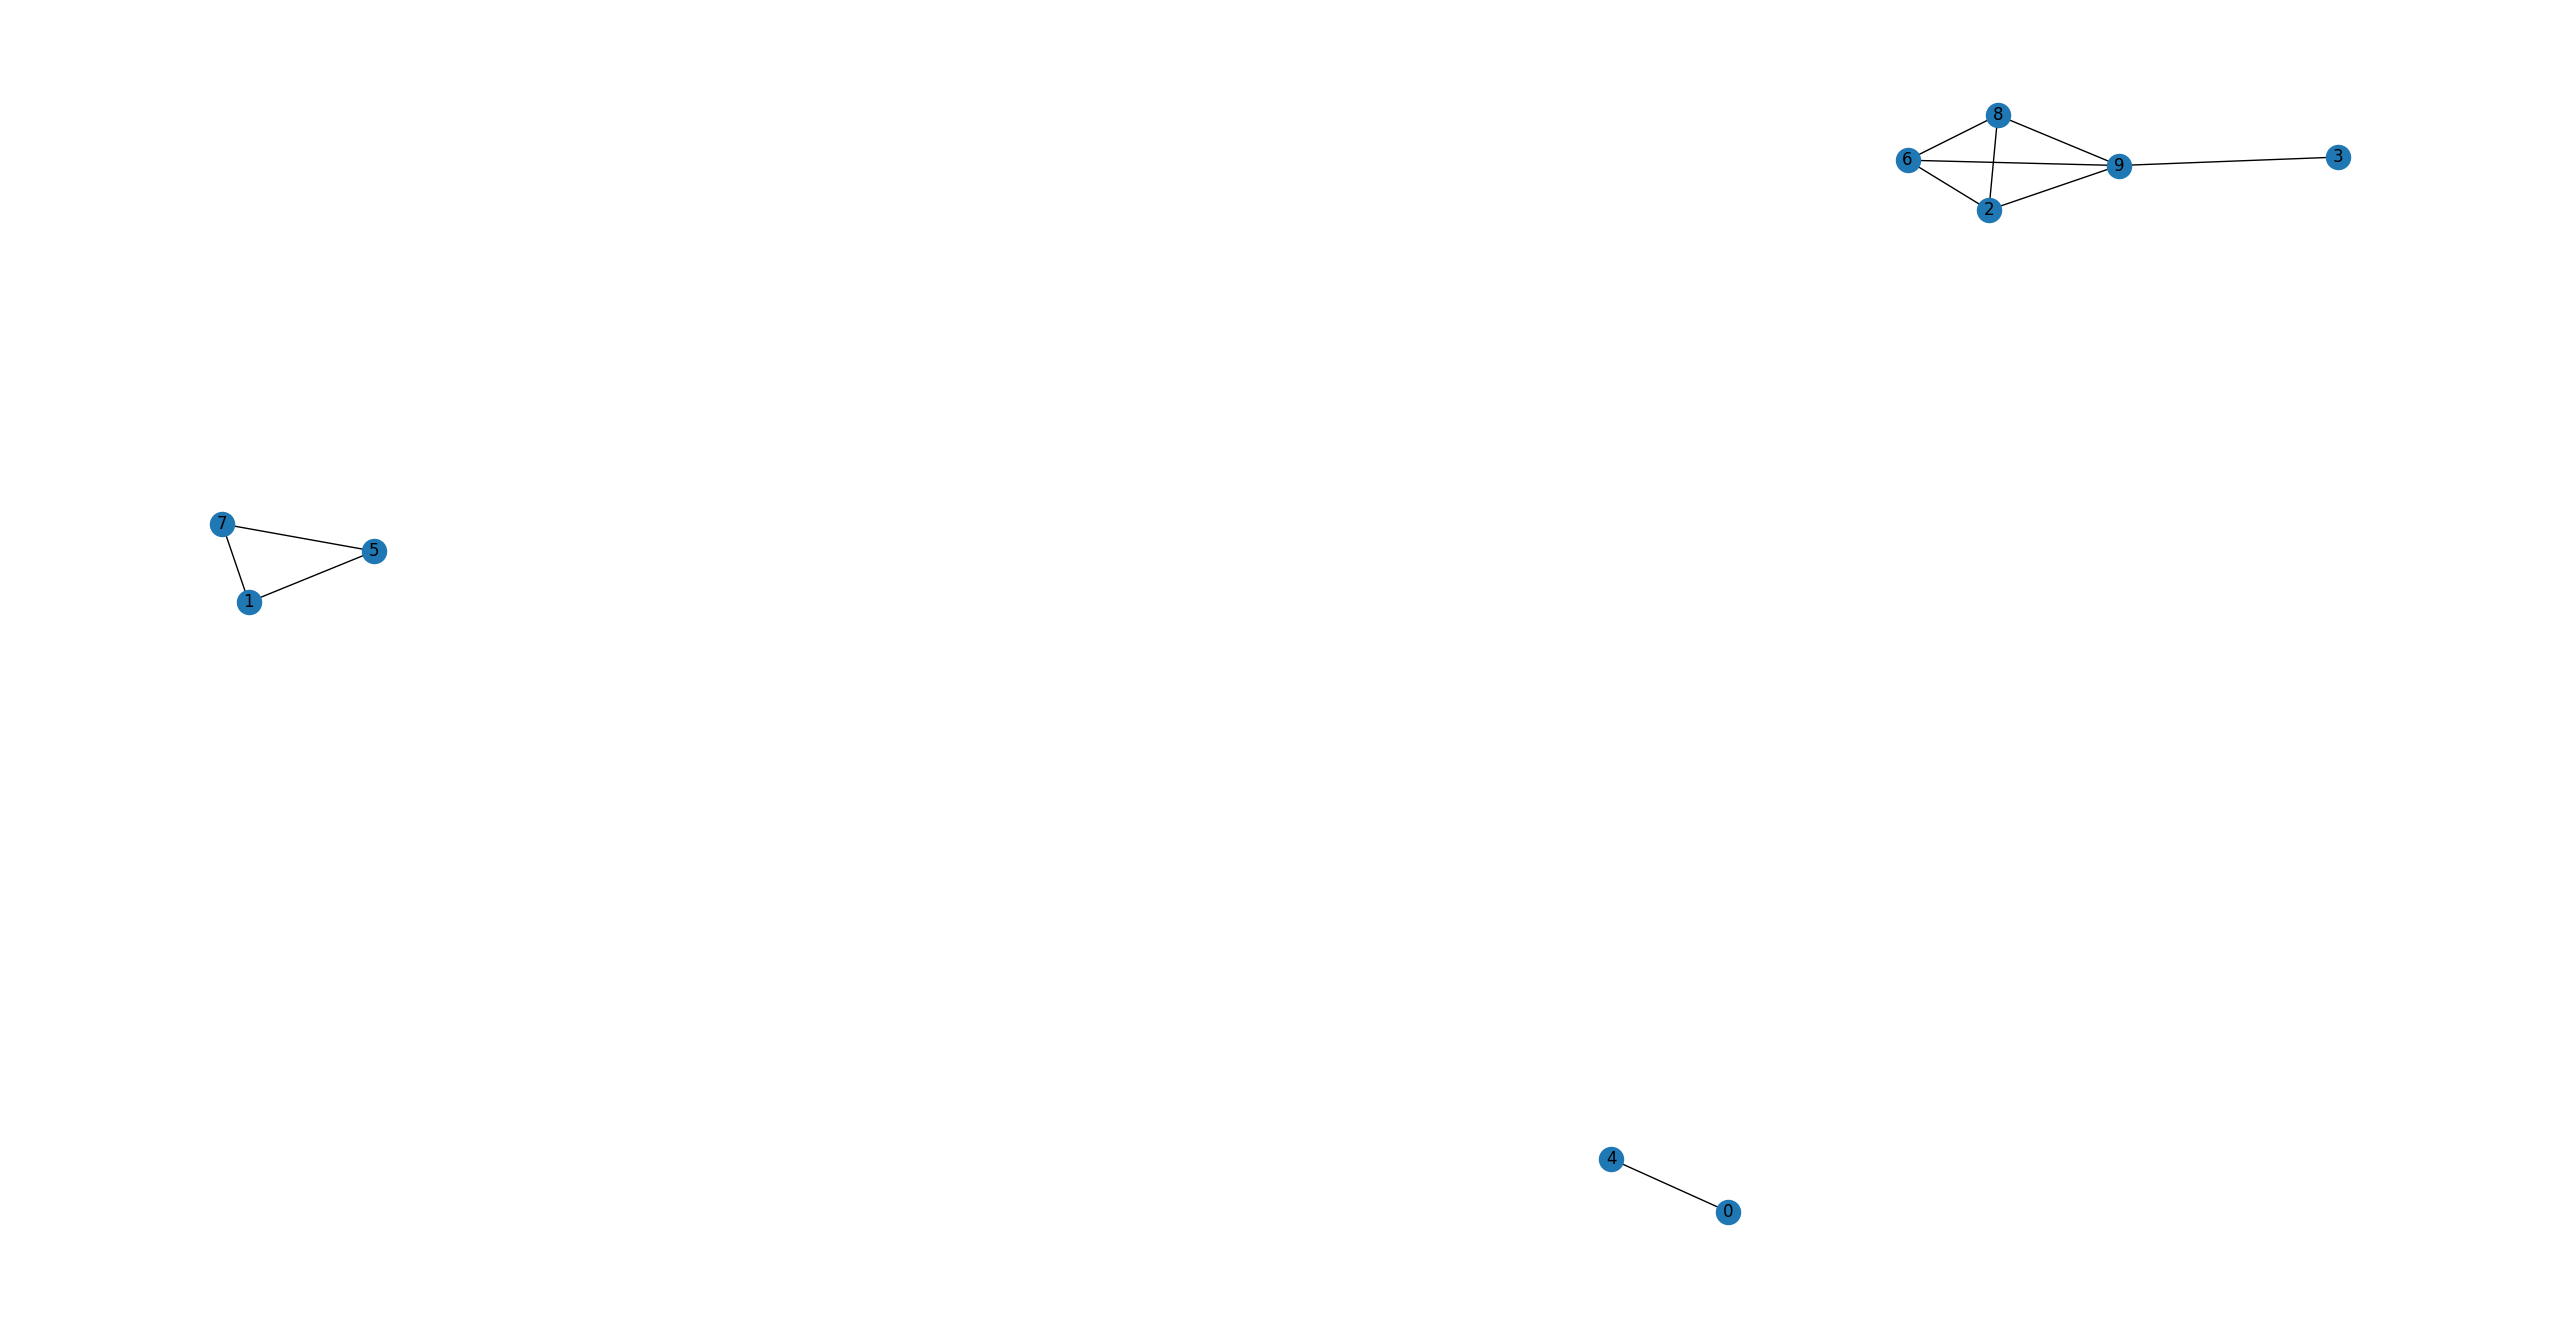
\includegraphics[width=\textwidth]{vr2.png}
        \caption{Randomly generated graph on 10 vertices.}\label{fig:vr2}
    \end{subfigure}
    \begin{subfigure}{0.33\linewidth}
        \centering
        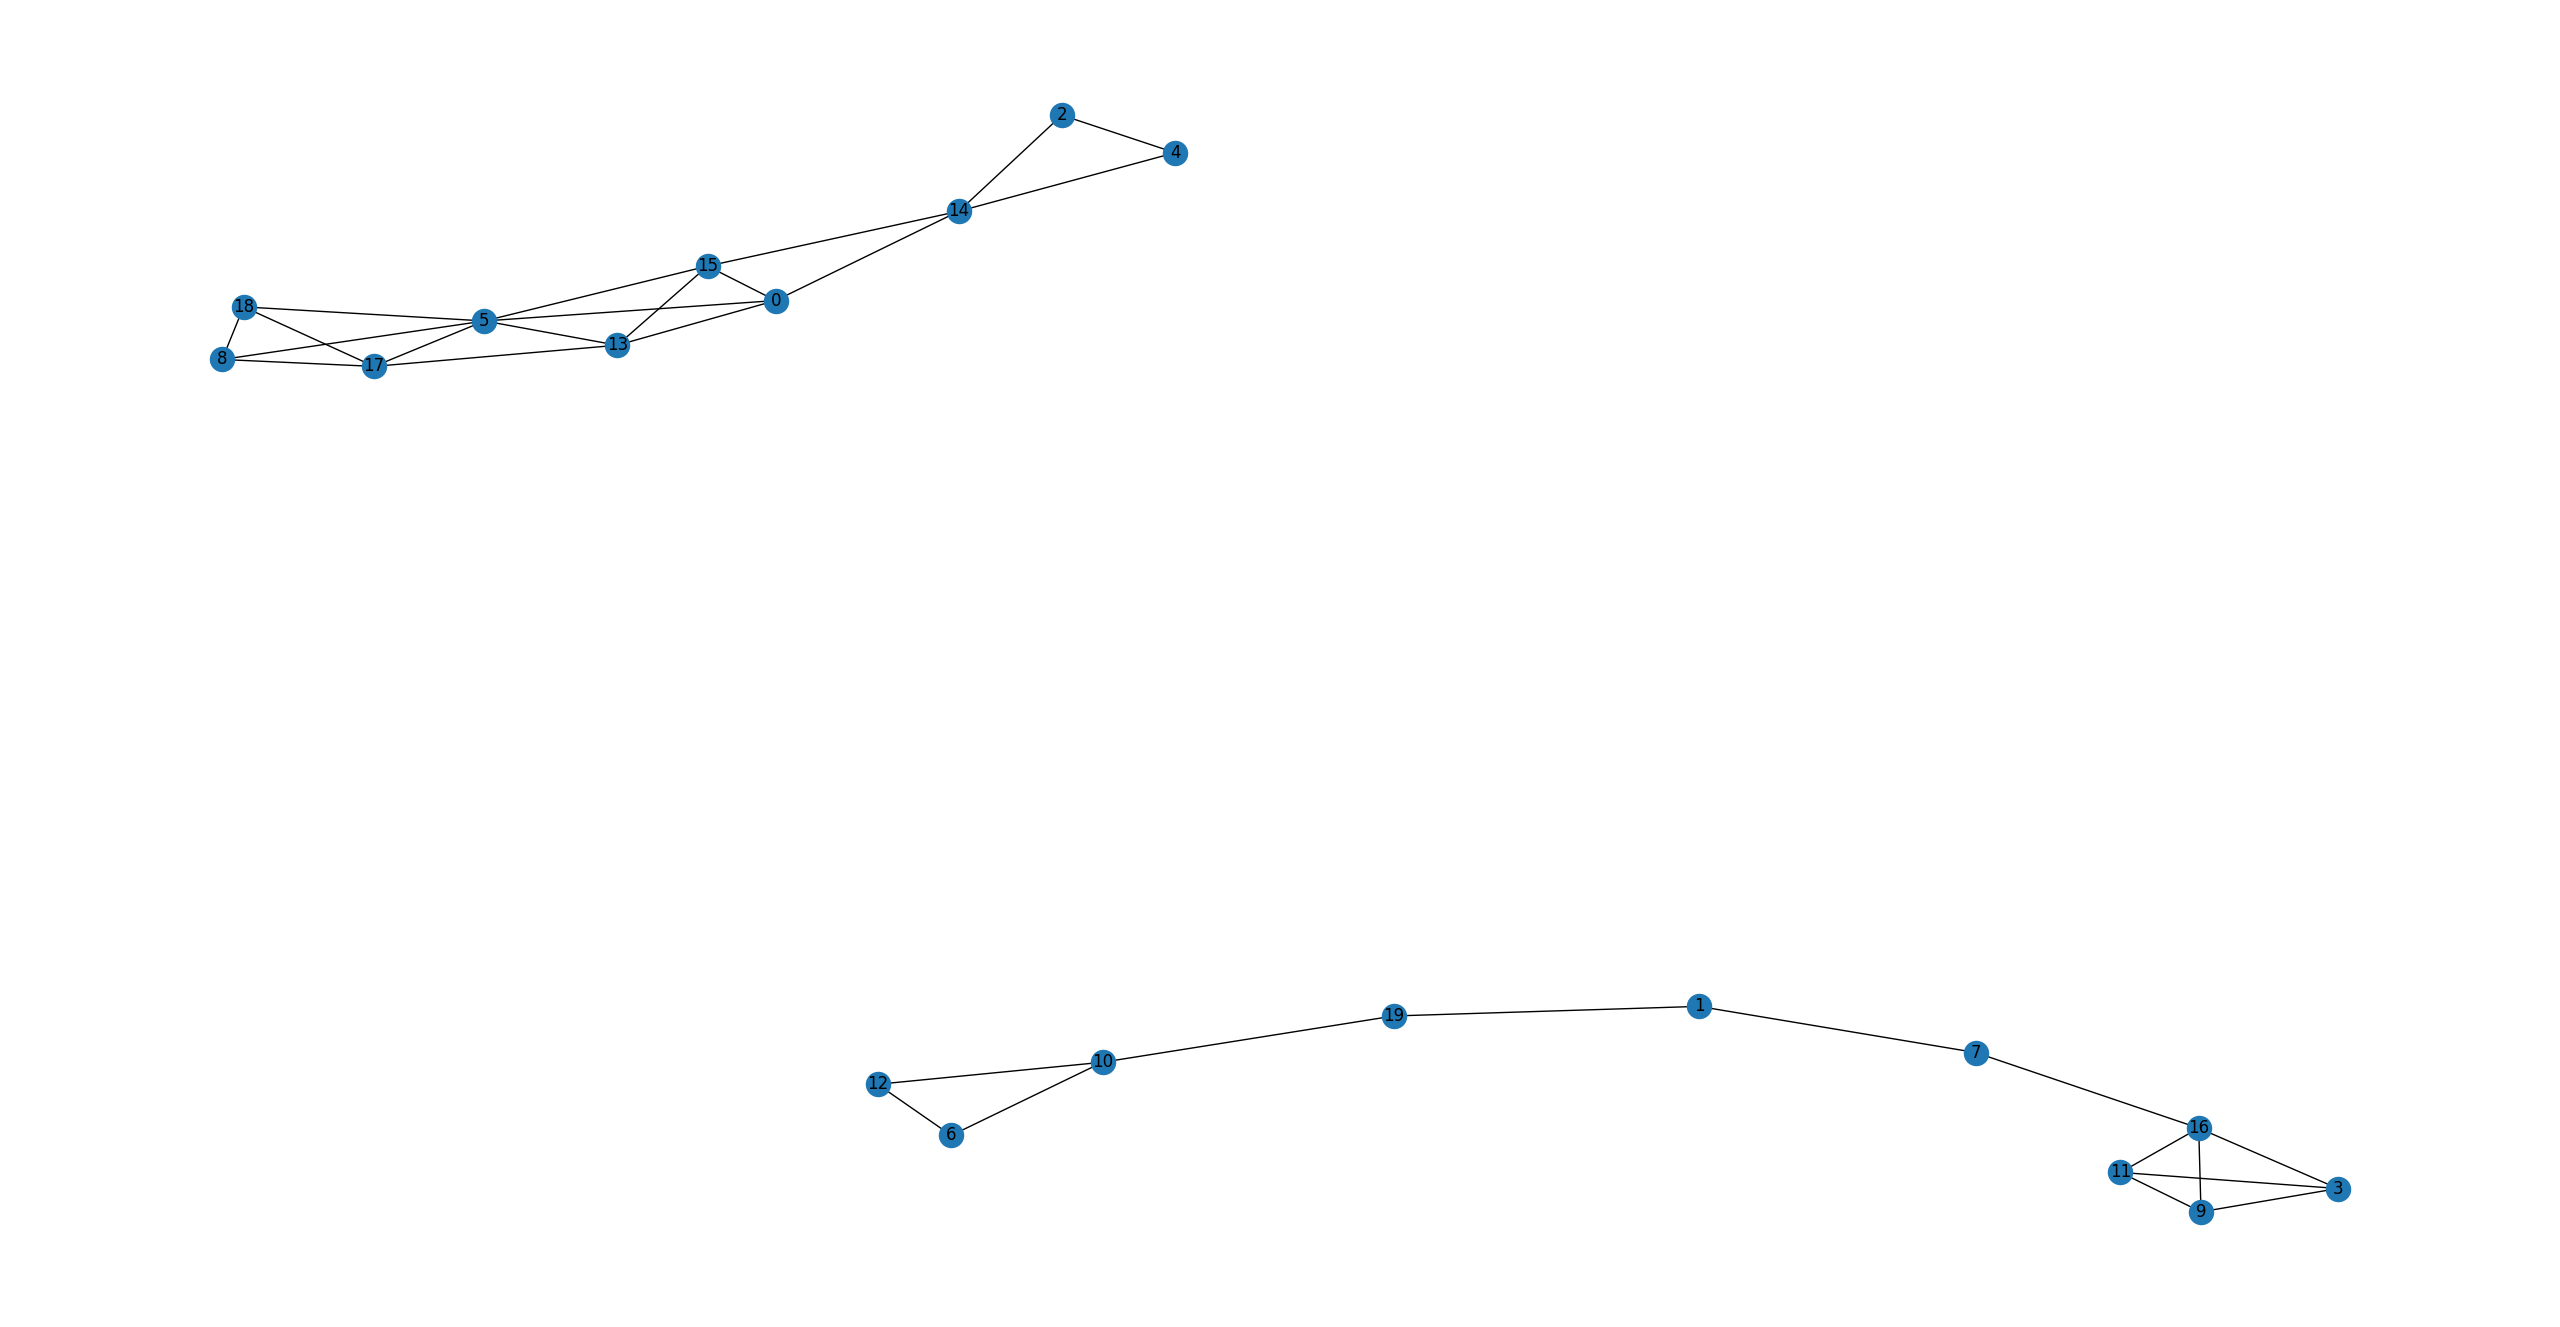
\includegraphics[width=\textwidth]{vr3.png}
        \caption{Randomly generated graph on 20 vertices.}\label{fig:vr3}
    \end{subfigure}
    \caption{Representation of input data used on Vietoris-Rips algorithm.}\label{fig:vrGraphs}
\end{figure}





\section{Čech complex}\label{sec:p4}

\section{Collapsibility}\label{sec:p5}

\end{document}
